\documentclass[lecture.tex]{subfiles}

\begin{document}

\exercice{}
%\video{https://youtu.be/blablabla}
\enonce{rdm-0022}{}

Nous considérons une poutre de longueur $4L$, en appui double et simple respectivement en $x=L$ (pivot) et $x=3L$ (ponctuelle). La poutre est soumise à deux forces ponctuelles $\vec{F}=-F \vec{y}$ en $x=0$ et $x=+4 L$. La section constante de la poutre est rectangulaire de hauteur $h$ et de largeur $b$. La poutre est en acier de module d'élasticité $E$ et de limite élastique $\sigma_{e}$. Le poids de la structure n'est pas prise en compte.

\medskip

On donne :

\begin{center}
  \begin{tabular}{|l|l|l|l|l|l|}
    \hline
    L = 400 mm & F = 800 N & b = 30 mm & h = 20 mm & E = 210 GPa & $\sigma_{e}$ = 450 MPa \\
    \hline
  \end{tabular}
\end{center}

\medskip

\begin{center}
  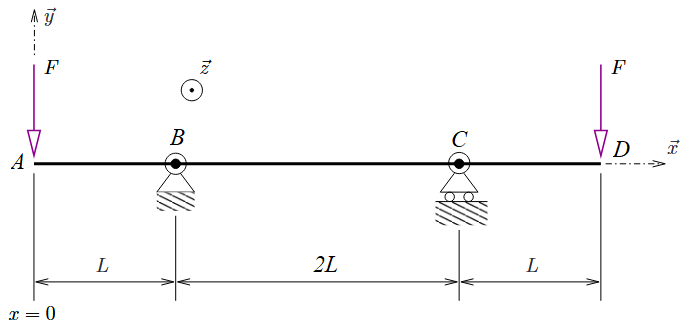
\includegraphics[scale=0.6]{figA0022.png}
\end{center}

\medskip

\begin{enumerate}
  \item Étudiez l’hyperstaticité du système.
  \item Calculez les actions de liaisons pour chaque appui sur la poutre. Faire les applications numériques.
  \item \label{itm:Q3}
  \begin{enumerate}
    \item Combien de coupe faut-il pour étudier les efforts internes du système ?
    \item Calculez analytiquement les expressions de l'effort tranchant interne $T(x)$ suivant la direction $\vec{y}$ et du moment fléchissant interne $M(x)$ suivant la direction $\vec{z}$ pour $x \in[0 ; 4L]$.
    \item Tracez les graphes de ces deux fonctions $T(x)$ et $M(x)$ pour $x \in[0 ; 4L]$ en précisant des valeurs numériques sur les axes.
    \item A quel(s) type(s) de flexion la poutre est-elle soumise?
  \end{enumerate}
  \item
  \begin{enumerate}
    \item Déterminez l'expression de la contrainte normale pour chacun des tronçons de la question \ref{itm:Q3} en fonction de l'abscisse $x$.
    %Déterminer l'expression de la contrainte normale dans la poutre. Sur un schéma d’une section, tracer son évolution. Préciser quelles points d’une section sont en traction, en compression. Déterminer cette contrainte (en fonction de l’abscisse $x$).
    \item Pour chacun des tronçons, sur le schéma d'une section, tracez l'allure de l'évolution de la contrainte normale et précisez les zones où les points subissent de la traction ou de la compression.
    %Pour les fibres supérieures de la poutre (pour y maximal), tracer l'évolution de cette contrainte normale le long de la poutre en fonction de l'abscisse $x$.
    \item Précisez le lieu (abscisse et position dans la section) où la contrainte normale est maximale, puis calculez la.
    \item Est-on encore dans le domaine élastique? Si oui, quel est le coefficient de sécurité?
  \end{enumerate}
  \item
  \begin{enumerate}
    \item Calculez l'expression de la flèche $y(x)$ pour $x \in[0 ; 4L]$. On précise que la symétrie du problème permet d'écrire que la déformation angulaire est nulle en $x=2L$, c'est à dire $y^\prime(2L)=0$. Afin de déterminer toutes les constantes d'intégration, on considérera les conditions de continuité pour $y$ et $y^\prime$.
    \item Tracez la déformée de la poutre, c'est à dire l'allure de $y(x)$.
    \item Evaluez numériquement la flèche maximale ainsi que sa position (en $x$).
  \end{enumerate}
\end{enumerate}

\finenonce{rdm-0022}
\finexercice

\end{document}
